\section{Engineering Shadow Reference Model (ESRM)}

\subsection{Overview}

The Engineering Shadow Reference Model (ESRM) defines the highest-level conceptual architecture of the Engineering Shadow platform.

Rather than describing implementation details, the ESRM explains how engineering information flows through the system and gradually evolves into meaningful engineering understanding.

The reference model serves as the conceptual foundation upon which all future architectural, implementation, and product decisions are based.

\vspace{0.4cm}

\begin{figure}[H]
    \centering
    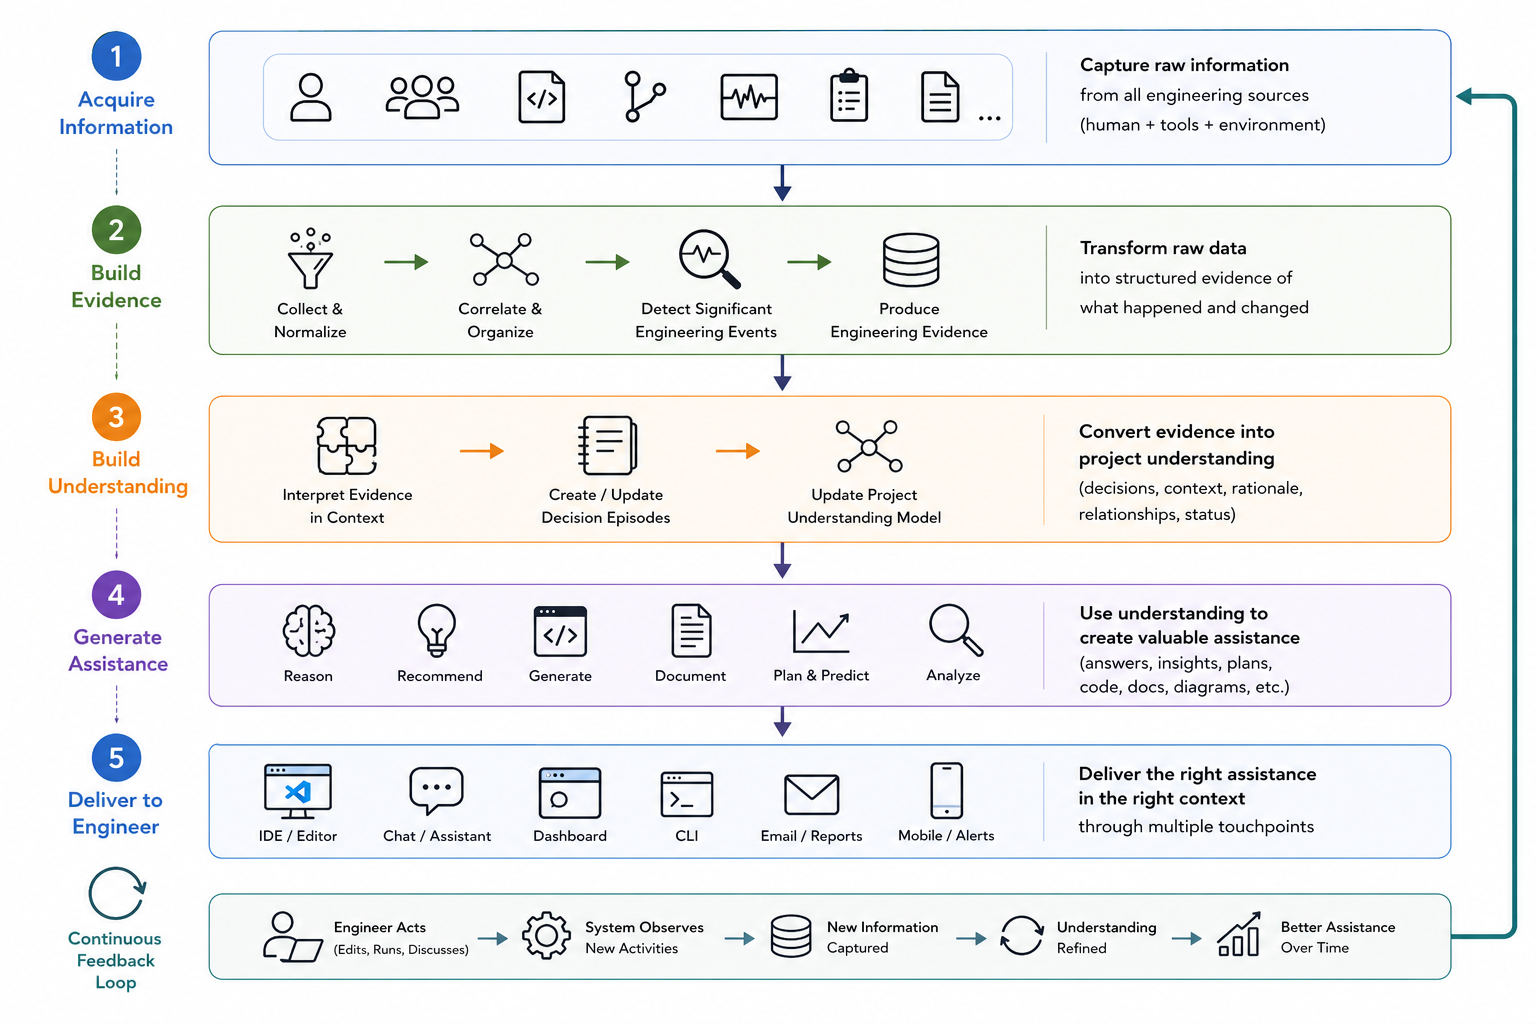
\includegraphics[width=\textwidth]{figures/conceptual/engineering_shadow_reference_model_v1.png}
    \caption{Engineering Shadow Reference Model Version 1}
    \label{fig:esrm}
\end{figure}

\subsection{Design Philosophy}

The architecture follows a simple principle:

\begin{center}

\textbf{Information $\rightarrow$ Evidence $\rightarrow$ Understanding $\rightarrow$ Assistance}

\end{center}

Rather than generating assistance directly from raw engineering activities, the system first constructs an evolving understanding of the project.

Engineering assistance is therefore generated from accumulated project understanding instead of isolated prompts or individual engineering events.

\vspace{0.4cm}

\subsection{Architecture Layers}

The ESRM consists of four conceptual layers.

\begin{enumerate}

\item Information Acquisition

Collect engineering information from both explicit and implicit sources including engineers, engineering tools, source code, documentation and project artifacts.

\item Evidence Construction

Transform raw engineering information into structured engineering evidence by correlating observations, detecting engineering events and filtering irrelevant activities.

\item Understanding Engine

Interpret engineering evidence to construct Decision Episodes and continuously maintain the Project Understanding Model (PUM).

\item Assistance Engine

Leverage the current Project Understanding Model to generate context-aware engineering assistance including recommendations, documentation, reasoning, planning and engineering insights.

\end{enumerate}

\vspace{0.4cm}

\subsection{Continuous Learning Loop}

Engineering Shadow operates as a continuously evolving system.

Every engineer interaction, engineering activity, design decision and project artifact contributes new information that refines the Project Understanding Model.

As project understanding improves, the quality of engineering assistance also improves.

\vspace{0.4cm}

\subsection{Architectural Significance}

The ESRM intentionally separates project understanding from engineering assistance.

This distinction enables multiple intelligent capabilities to share a common understanding of the project while remaining independent of individual user interfaces, AI models or implementation technologies.

Consequently, the Project Understanding Model becomes the central knowledge asset of the Engineering Shadow platform.
